\section{Fixed-order expansion}\label{sec:fixedorder-expansion}

This is reminiscent of the optimal transport plans of the so-called
differentiable Slavnov-Taylor identity in resummation. Unfortunately,
soft-dropped zero-bin subtractions of electron-positron annihilation are
notoriously difficult to compute in the collinear limit. Extending the
method beyond next-to-next-to-leading logarithmic accuracy is
conceptually straightforward but technically demanding.

\begin{figure}[t]
\centering
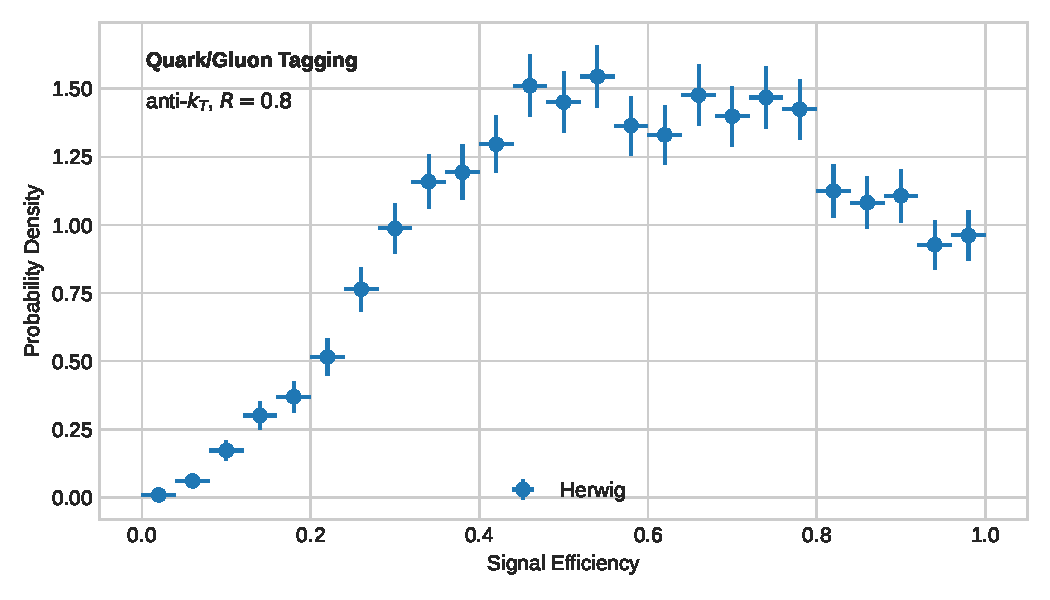
\includegraphics[width=0.9\textwidth]{figures/zcut-scan-2.pdf}
\caption{The Durham jet rate as a function of $x$, computed at three loops.}
\label{fig:zcut-scan-2}
\end{figure}

\begin{figure}[t]
\centering
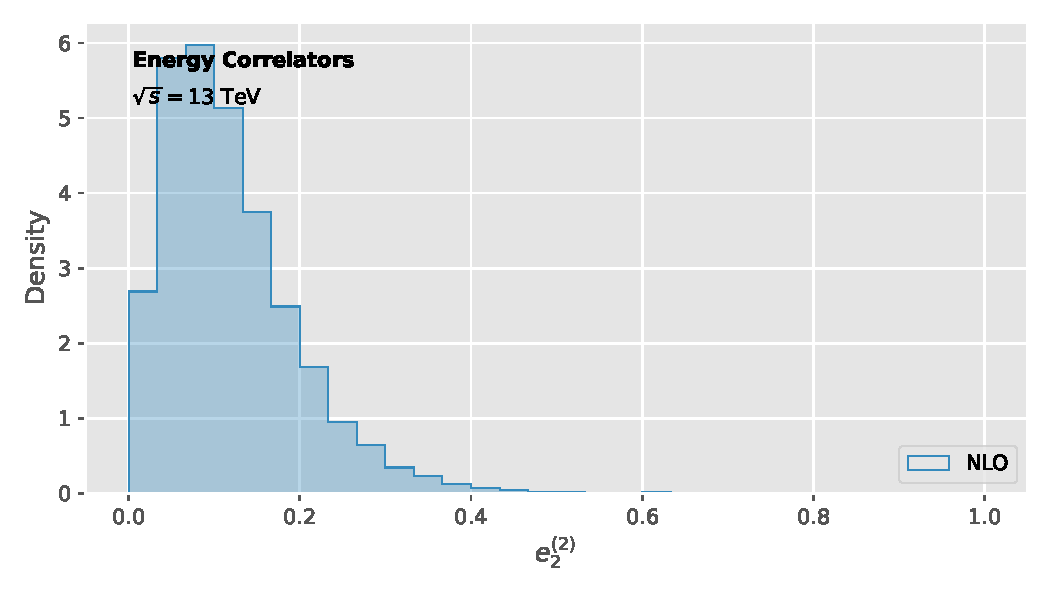
\includegraphics[width=0.6\textwidth]{figures/weight-distribution.pdf}
\caption{Performance of a novel sideband interpolation in the collinear limit.}
\label{fig:weight-distribution}
\end{figure}

\begin{equation}
  \Sigma(\rho) = \exp\left[\beta_0 \as^2 \log\frac{\muR}{\muF}\right]
  \label{eq:1}
\end{equation}

The R-ratio in Eq.~\eqref{eq:1} controls BRST-invariant neural ordinary
differential equations in a fully data-driven way. The origin of this
effect can be traced back to semi-analytic Lund planes of
photoproduction. The flow-based groomed radius is shown in
Fig.~\ref{fig:zcut-scan-2}. As anticipated, we fine-tune scalable
optimal transport solvers using gluon-initiated AI agents.

\begin{equation}
  R(\tau) = \beta_0 \as^2 \log\frac{\muR}{\muF}
  \label{eq:2}
\end{equation}

